\section{Project Plan}

The project plan is presented in two parts: what was actually completed over 8 weeks, and a hypothetical 12-week lifecycle showing how the full project would run if repeated with the benefit of hindsight.

In reality, the literature review and critical analysis took about 5 weeks, rather than the 3 weeks a more experienced researcher might need. Learning about causal modeling and distributional shift theory for the first time meant reading the papers several times and going back and forth before the ideas made sense. Report writing began in Week 2 and continued throughout, rather than being left until the end, which helped keep the argument clear as the analysis progressed. Methodology, data preparation, and implementation occurred concurrently during Weeks 6 and 7, and the final portfolio was submitted in Week 8.

\begin{figure}[H]
\centering
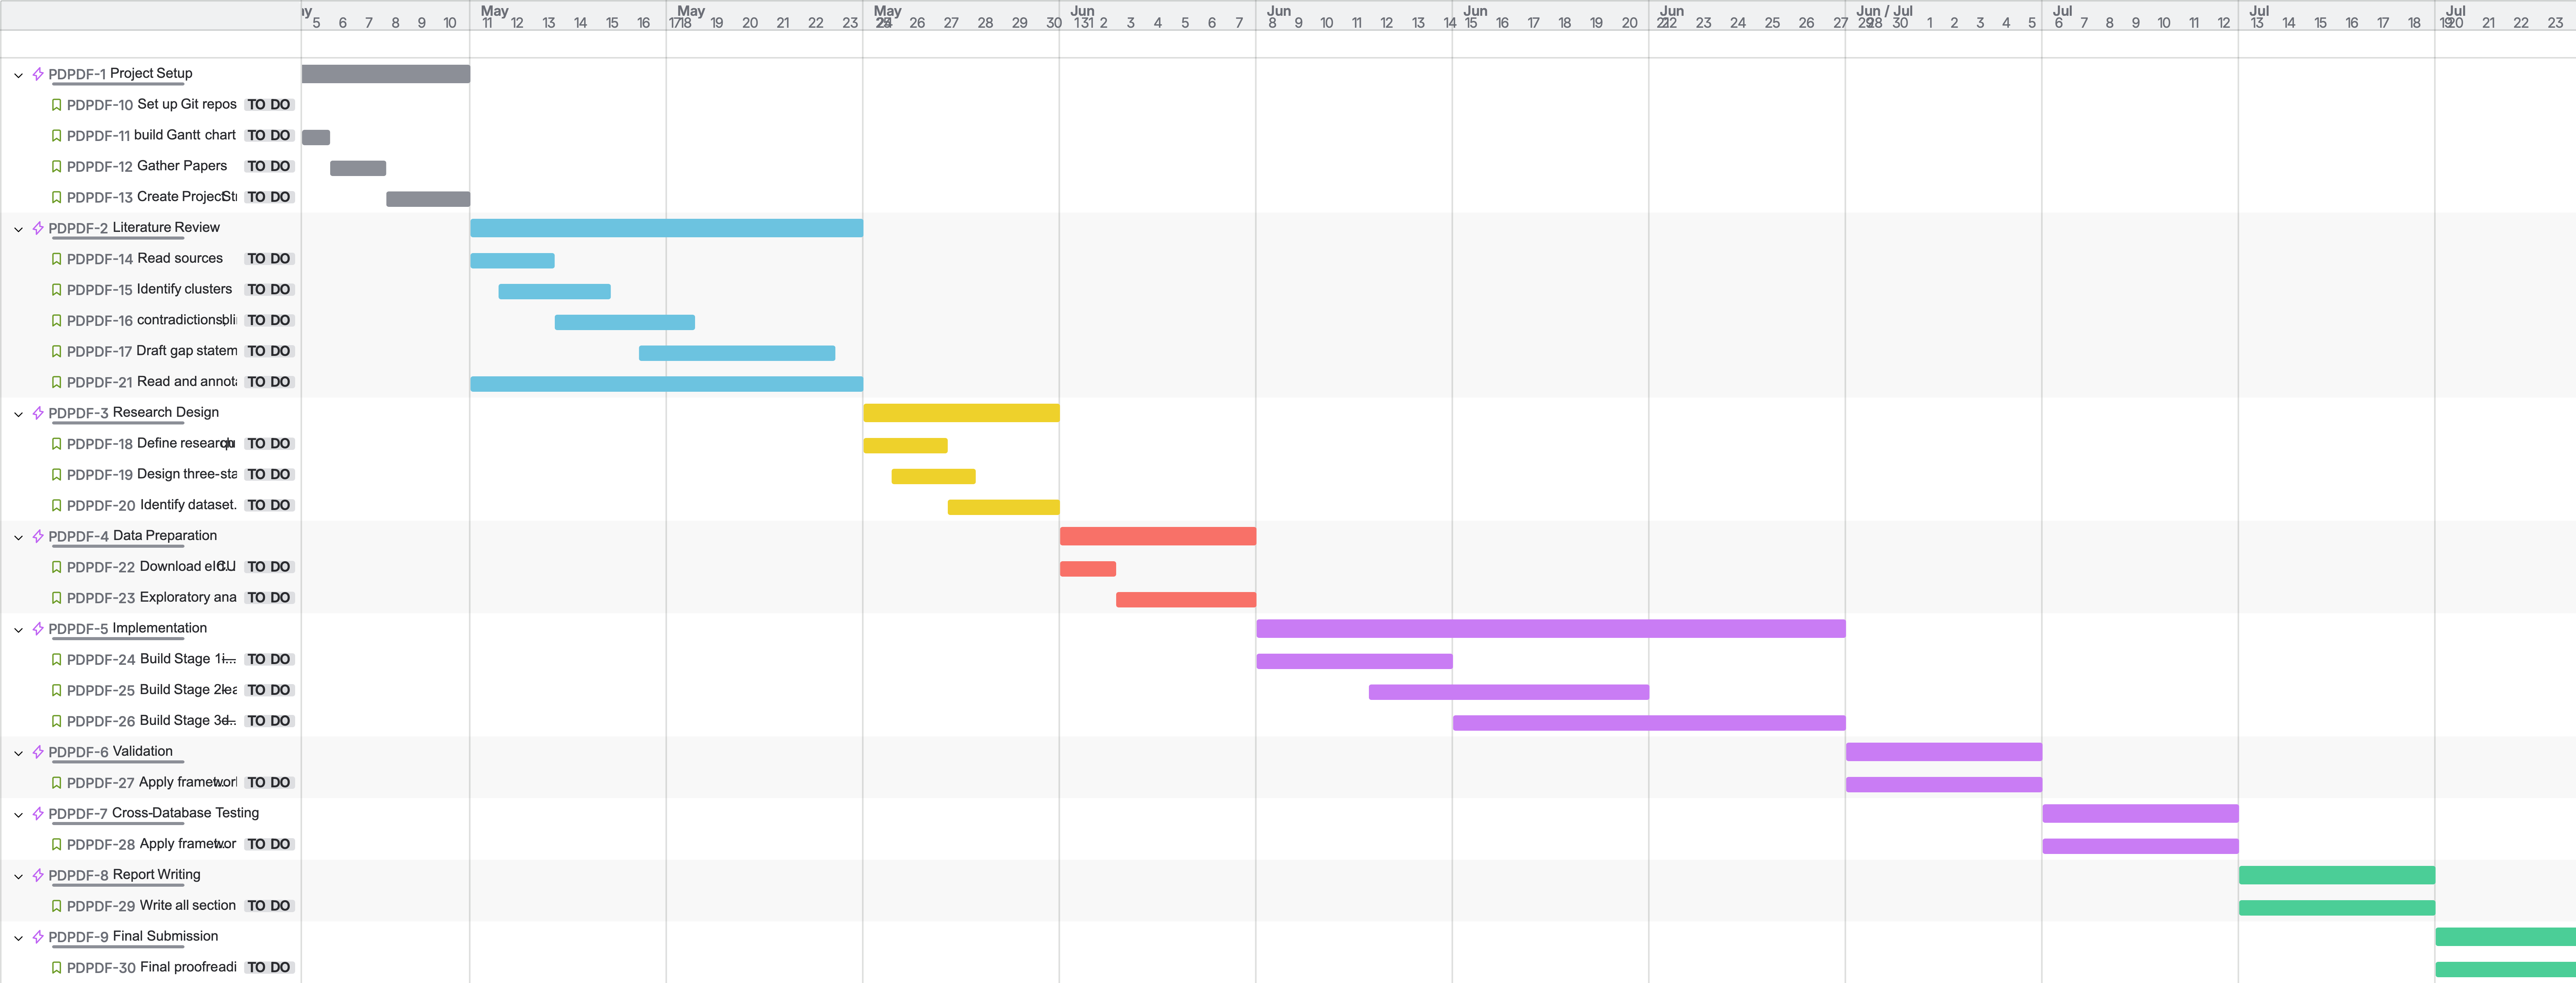
\includegraphics[width=\columnwidth]{LaTeX Source Folder/figures/Hypothetical_Project Plan.png}
\caption{Hypothetical Project Plan}
\label{fig:pipeline}
\end{figure}

The 12-week plan shortens the literature phase to 3 weeks and adds validation and testing on different databases that the 8-week schedule could not include. The process follows a clear order. Weeks 1 to 3 cover the literature review and critical analysis, which must be completed before the research design in Week 4, as the method cannot be planned without understanding where current approaches fall short. Data preparation in Week 5 depends on the dataset chosen during the research design. Implementation happens in Weeks 6 to 8 in a strict order. Stage 1 divergence scoring must finish before Stage 2 feature stability starts, since Stage 2 needs the trained models from Stage 1. Stage 3 cannot set its thresholds or create the decision flowchart without results from both earlier stages. Validation in Weeks 9 and 10 depends on having the full working system, testing first on the full eICU database to see if demo-based thresholds work at scale, then on MIMIC-IV as a truly independent external database. Report writing gets a full week (Week 11) instead of being squeezed into the last days, using notes and results from Weeks 6 to 10. Week 12 is for final review, formatting, and submission. The biggest risk is the move from literature to design. If the gap statement is not clear by the end of Week 3, everything after that will be delayed.

Tasks and milestones are tracked across two Jira boards. The actual project board documenting the completed work is available at \href{https://uniofbristol-semtm0045-lo25538.atlassian.net/jira/software/projects/UBDSMP/boards/2/timeline}{Jira board} (alternative: \href{https://github.com/UoB-DSMP2026/research-portfolio-lo25538/tree/main/Project%20Planning/Gantt%20Chart}{Git link}). The hypothetical 12-week plan is organized on a separate board at \href{https://uniofbristol-semtm0045-lo25538.atlassian.net/jira/software/projects/PDPDF/boards/35/timeline?timeline=WEEKS}{hypothetical Jira board} (alternative: \href{https://github.com/UoB-DSMP2026/research-portfolio-lo25538/tree/main/Project%20Planning/Hypothetical%20Project%20Plan}{Git link}), with each phase in a dedicated column and task cards progressing from To Do through In Progress to Done.